\documentclass[12pt,a4paper]{article}

\usepackage{csquotes}
\usepackage{algpseudocode}
\usepackage{algorithm}
\usepackage{amsfonts}
\usepackage{caption}
\usepackage{ amssymb }
\usepackage{amsmath}
\usepackage{breqn}
\usepackage{pgf}
\usepackage{blindtext}
\usepackage{hyperref}
\usepackage[T1]{fontenc} % Use 8-bit encoding that has 256 glyphs
\usepackage{mathtools}
\graphicspath{{images}}
\renewcommand{\algorithmicrequire}{\textbf{Parameters:}}
\renewcommand{\algorithmicensure}{\textbf{Initialization:}}
\newcommand{\defeq}{\vcentcolon=}
\newcommand{\eqdef}{=\vcentcolon}
\algnewcommand{\Inputs}[1]{%
	\State \textbf{Inputs:}
	\Statex \hspace*{\algorithmicindent}\parbox[t]{.8\linewidth}{\raggedright #1}
}
\algnewcommand{\Initialize}[1]{%
	\State \textbf{Initialize:}
	\Statex \hspace*{\algorithmicindent}\parbox[t]{.8\linewidth}{\raggedright #1}
}
\begin{document}

\title{%
Multi-Agent Learning:\\From Theory to Practice \\
	\large Report of \enquote{The Non Stochastic Multi-Armed Bandit Problem}}
\author{Carlos Alberto Santillán Moreno, M.Sc. student}
\date{July 15th 2023}
\maketitle	

\section{Summary}

The paper \cite{j18} tackles the \textit{adversarial} multi-armed bandit problem. In this context, an agent is presented with $K$ different arms, but their rewards are not drawn from fixed distributions (for a thorough analysis in the stochastic case, see Auer et al. \cite{regretstat}). Instead, each arm has been assigned a sequence of rewards, i.e., one reward for each round $t$.  The reward of the $i$-th arm at round $t$ is denoted as $x_i(t)$. We aim to minimize the \textit{weak regret} over the time horizon $T$,  which is the difference between $G_{\max}(T)$, the cumulative reward of the globally best single action, and $G_{A}(T)$, the cumulative reward of algorithm $A$. The adversarial setting was originally presented in Auer et al. \cite{original}. The main algorithm proposed in the paper is \textbf{Exp3} (see Algorithm \ref{alg:Exp3}).

\begin{algorithm}
	\caption{\textbf{Exp3}}\label{alg:Exp3}
	\begin{algorithmic}[1]         
		\Require{ Real $\gamma$ $\in$ (0,1] }
		\Ensure{ $w_i(1) = 1$ for $i = 1,\dots, K$ }
		\For{$t = 1, 2, \dots$}
		\State Set $p_i(t) = (1-\gamma)\frac{w_i(t)}{\sum_{j=1}^{K}w_j(t)}+\frac{\gamma}{K}$ for $i = 1,\dots, K$
		\State Draw $i_t$ randomly according to the probabilities $p_1(t), \dots, p_K(t)$
		\State Receive reward $x_{i_t}(t) \in [0, 1]$
		\State{\textbf{for} $j = 1,\dots,K$ \textbf{do}} 
		\[ \hat{x}_j(t) =\begin{cases} 
			x_j(t)/p_j(t) & \text{if} \,\, j = i_t \\
			\,\,\,\,\,\,\,\,\,\,\,\,0 & \text{otherwise} 
		\end{cases}
		\]
		\begin{align*}
			w_j(t + 1) = w_j(t)\exp(\gamma\hat{x}_j(t)/K)
		\end{align*}
		\State{\textbf{end for}}
		\EndFor
	\end{algorithmic}
\end{algorithm}
The idea behind \textbf{Exp3}, and all of its variants, is to update the probability $p_i(t)$ of pulling arm $i$ if the arm is promising. We start from a uniform distribution since all weights are equal to 1, therefore all arms are equally likely to be chosen. At each round $t$ we pull an arm according to the probabilities $p_1(t),\dots, p_K(t)$ and get a reward $x_{i_t}(t)$. We introduce the estimated reward $\hat{x}(t)$, which is  zero for all arms that were not pulled at round $t$, and $x_j(t)/p_j(t)$ for the pulled arm. The factor $1/p_j(t)$ compensates for the probability of taking that action. This guarantees that $\mathbb{E}[\hat{x}_j(t)|i_1,\dots, i_{t-1}] = x_j(t)$, i.e., expectations are equal to the actual reward for each action. The last step is updating the weights by an exponential factor $\gamma\cdot \hat{x}_j(t)/K$, which will make the algorithm more likely to choose arms with higher rewards (i.e., the more promising ones). By assigning different probabilities to each arm we try to balance exploration and exploitation, so it is still possible to pull less promising arms, albeit with a lower probability.
It can be proven that by a proper choice of the parameter $\gamma$ the \textit{expected} weak regret of \textbf{Exp3} is ${O}(\sqrt{gK\ln K})$, where $g \geq G_{\max}$\footnote{Assuming rewards in the range $[0,1]$ we can set $g = T$, which requires knowledge of $T$}. 

\textbf{Exp3} can be further modified to  work without knowledge of $T$, provide more guarantees on the regret bound, or both.  The paper presents \textbf{Exp3.1}, which is designed to work without knowing $T$. \textbf{Exp3.1} "guesses" $g$ and calls \textbf{Exp3}.  When the \textit{estimated} cumulative reward of an arm is larger than $g$, \textbf{Exp3.1} restarts \textbf{Exp3} with an updated $g$ (each restart corresponds to an epoch). \textbf{Exp3.1} has a regret of ${O}(\sqrt{KT\ln K})$, which in general can be worse than \textbf{Exp3}.

A problem of \textbf{Exp3} is that its expected regret has a large variance, because the estimated rewards $\hat{x}_i(t)$  can have a variance close to ${1}/{p_i(t)}$, which can lead to a regret variance as large as $T^{3/4}$. 
\textbf{Exp3.P} addresses this by using confidence bounds on the estimated cumulative reward, which leads  to a  \textit{weak regret} (not its expectation)  of ${O}(\sqrt{KT\ln(KT/\delta)})$ with probability at least $1-\delta$. Using a similar approach to \textbf{Exp3.1} we can obtain \textbf{Exp3.P.1}, which does not require knowledge of $T$, and also keeps the variance under control. 

Another variant is \textbf{Exp4}, we rely on "expert" advice, experts are defined as a probability distribution over the actions at each round, so we choose the most promising expert rather than the arm itself.  The last variant, \textbf{Exp3.S}, generalizes the regret against any sequence of actions $(j_1,\dots,j_T)$, not only the globally best single action.  However, the bound on the expected regret depends on the "hardness" of the sequence, where the hardness is the number of times one has to change the arm to follow the sequence plus 1.

\section{Technical Evaluation}

We provide a short version of the proof of the upper bound of the expected regret of \textbf{Exp3}. 
\\\\
\textbf{Theorem 2.1}	\textit{For any $K > 0$ and for any $\gamma \in (0,1]$} 
	\begin{align*}
		G_{\max}-\mathbb{E}[G_{\textbf{Exp3}}] \leq (e-1)\gamma G_{\max}+\frac{K\ln K}{\gamma}
	\end{align*}
	\textit{holds for any assignment of rewards and for any $T > 0$}
\\\\
Let $W_t = w_1(t)+ \dots +  w_K(t)$. We bound the ratio $W_{t+1}/W_t$ for all sequences $i_1,\dots,i_T$ drawn by \textbf{Exp3}.

\begin{align*}
		\frac{W_{t+1}}{W_t}={}& \sum_{i=1}^{K}\frac{w_i(t+1)}{W_t}\\
			     ={}& \sum_{i=1}^{K}\frac{p_i(t)-\frac{\gamma}{K}}{1-\gamma}\exp\bigg(\frac{\gamma}{K}\hat{x}_i(t)\bigg)\\
			     \leq{}& 1+ \frac{\frac{\gamma}{K}}{1-\gamma}x_{i_t}(t)+\frac{(e-2)(\frac{\gamma}{K})^2}{1-\gamma}\sum_{i=1}^{K}\hat{x}_i(t).
\end{align*}
By taking the logarithm of the ratio and remembering some well-known inequalities we obtain
\begin{align*}
	\ln \frac{W_{t+1}}{W_{t}}\leq \frac{\frac{\gamma}{K}}{1-\gamma}x_{i_t}(t) + \frac{(e-2)(\frac{\gamma}{K})^2}{1-\gamma}\sum_{i=1}^{K}\hat{x}_i(t)
\end{align*}
Summing over $t$ we get
\begin{align*}
		\ln \frac{W_{T+1}}{W_1} \leq \frac{\frac{\gamma}{K}}{1-\gamma}G_{\textbf{Exp3}} + \frac{(e-2)(\frac{\gamma}{K})^2}{1-\gamma} \sum_{t=1}^{T}\sum_{i=1}^{K}\hat{x}_i(t)
\end{align*}
We know that for any action $j$
\begin{align*}
	\ln \frac{W_{T+1}}{W_1} \geq \ln \frac{w_j(T+1)}{W_1} = \frac{\gamma}{K}\sum_{t=1}^{T}\hat{x}_j(t)-\ln K
\end{align*}
By subtracting the last two expressions we obtain 
\begin{align*}
	G_{\textbf{Exp3}} \geq (1-\gamma)\sum_{t=1}^{T}\hat{x}(t)-\frac{K\ln K}{\gamma}-(e-2)\frac{\gamma}{K}\sum_{t=1}^{T}\sum_{i=1}^{K}\hat{x}_i(t)
\end{align*}
We can take the expection on both sides w.r.t. the distribution of the chosen arms,  we get
\begin{align*}
		\mathbb{E}[G_{\textbf{Exp3}}] \geq (1-\gamma)\sum_{t=1}^{T}x_j(t)-\frac{K\ln K}{\gamma}-(e-2)\frac{\gamma}{K}\sum_{t=1}^{T}\sum_{i=1}^{K}x_i(t)
\end{align*}
where we exploited the fact that $\mathbb{E}[\hat{x}_j(t)|i_1,\dots,i_{t-1}] = x_j(t)$. Considering that we chose the action $j$ arbitrarily, and that
\begin{align*}
	\sum_{t=1}^{T}\sum_{i=1}^{K}x_i(t)\leq K G_{\max}
\end{align*}
we obtain the inequality stated by the theorem. \,\,\,\,\,\,\,\, $\blacksquare$

All the bounds presented in the paper are proven following a similar reasoning. In particular, they make use of the following observations
\begin{gather*} 
	\hat{x}_i(t) \leq 1/p_i(t) \leq K/\gamma,  \\
	\sum_{i=1}^{K}p_i(t)\hat{x}_i(t) = p_{i_t}(t)\frac{x_{i_t}(t)}{p_{i_t}(t)} = x_{i_t}(t),\\
	\sum_{i=1}^{K}p_i(t)\hat{x}_i(t)^2=p_{i_t}(t)\frac{x_{i_t}(t)}{p_{i_t}(t)}\hat{x}_{i_t}(t) \leq \hat{x}_{i_t}(t)= \sum_{i=1}^{K}\hat{x}_i(t).
\end{gather*}

The paper also presents proofs for the optimality of parameters such as $\gamma$, or also $\alpha$ in \textbf{Exp3.P}. 

The assumptions made are as general as possible for the adversarial setting. For example, we assume that rewards belong to the interval $[0,1]$. However, this does not limit the generalization of the algorithms presented. We can consider any reward interval $[a,b]$ (with $a < b$) by scaling the rewards accordingly
\begin{align*}
	\frac{x_j(t) - a }{b - a}
\end{align*}  
so we end up with a $[0,1]$ interval. This obviously requires knowledge of the interval.

To corroborate the findings outlined in the paper, we present the results obtained by a Python implementation\footnote{The code is available at this repository \url{https://github.com/Plinkett/MALReport}} of some of the algorithms.
We consider binary rewards, 10 arms, and $T = 100000$. The rewards for each arm were assigned at each round with these probabilities [0.30, 0.28, 0.26, 0.24, 0.22, 0.19, 0.17, 0.15, 0.14, 0.10], so the best arm is the first one. We show the performance of \textbf{Exp3} with the optimal $\gamma$ (Figure 1).

\begin{figure}[!htb]
	\begin{center}
		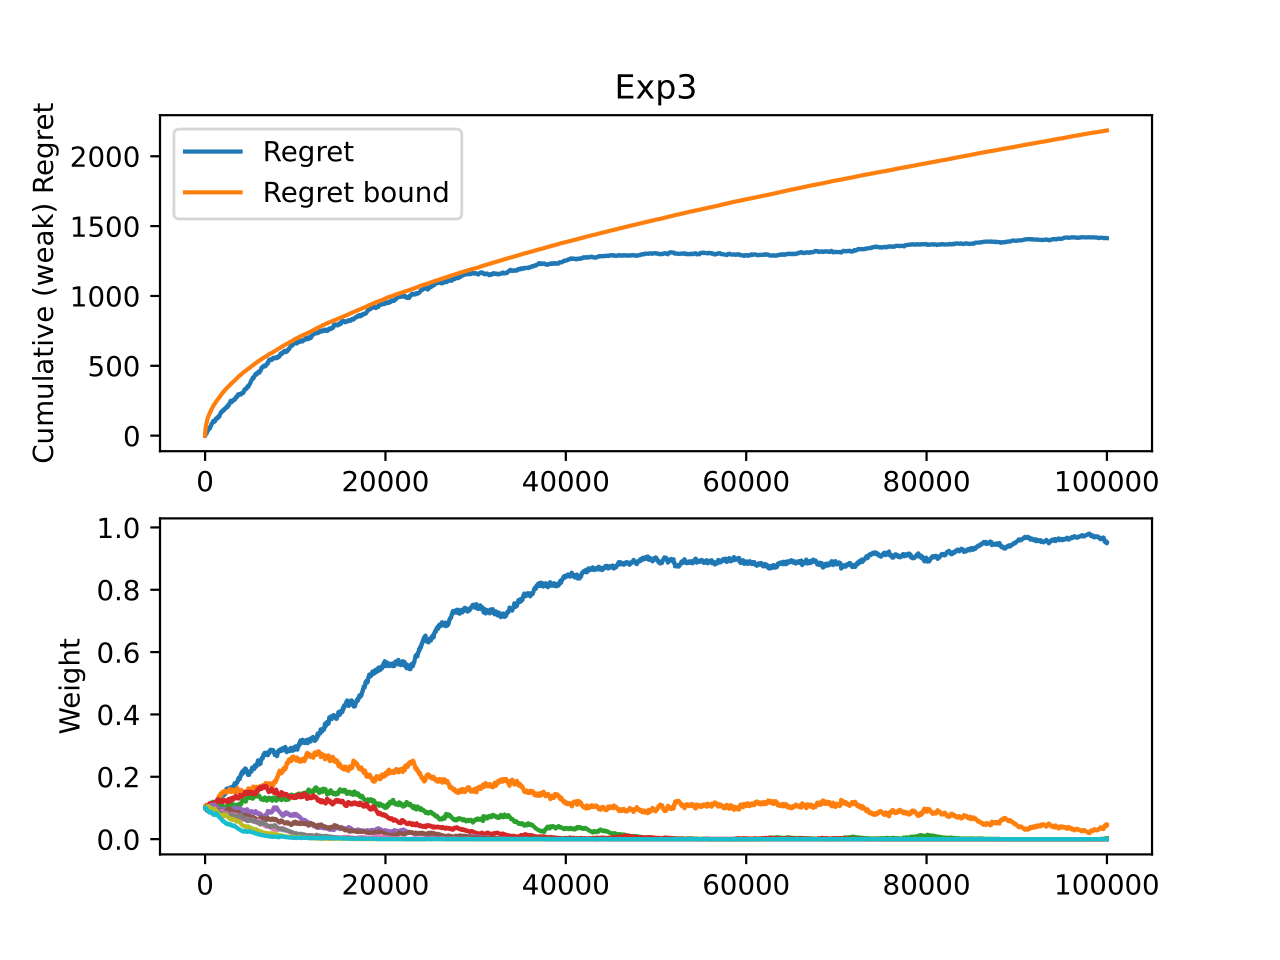
\includegraphics[width=90mm, height=70mm]{exp3optimal.png}
		\caption{Cumulative regret and weights of \textbf{Exp3} over the time horizon}
	\end{center}
\end{figure}

We now show the performance of \textbf{Exp3.1} on the same dataset of rewards (Figure 2). 

\begin{figure}[!htb]
	\begin{center}
		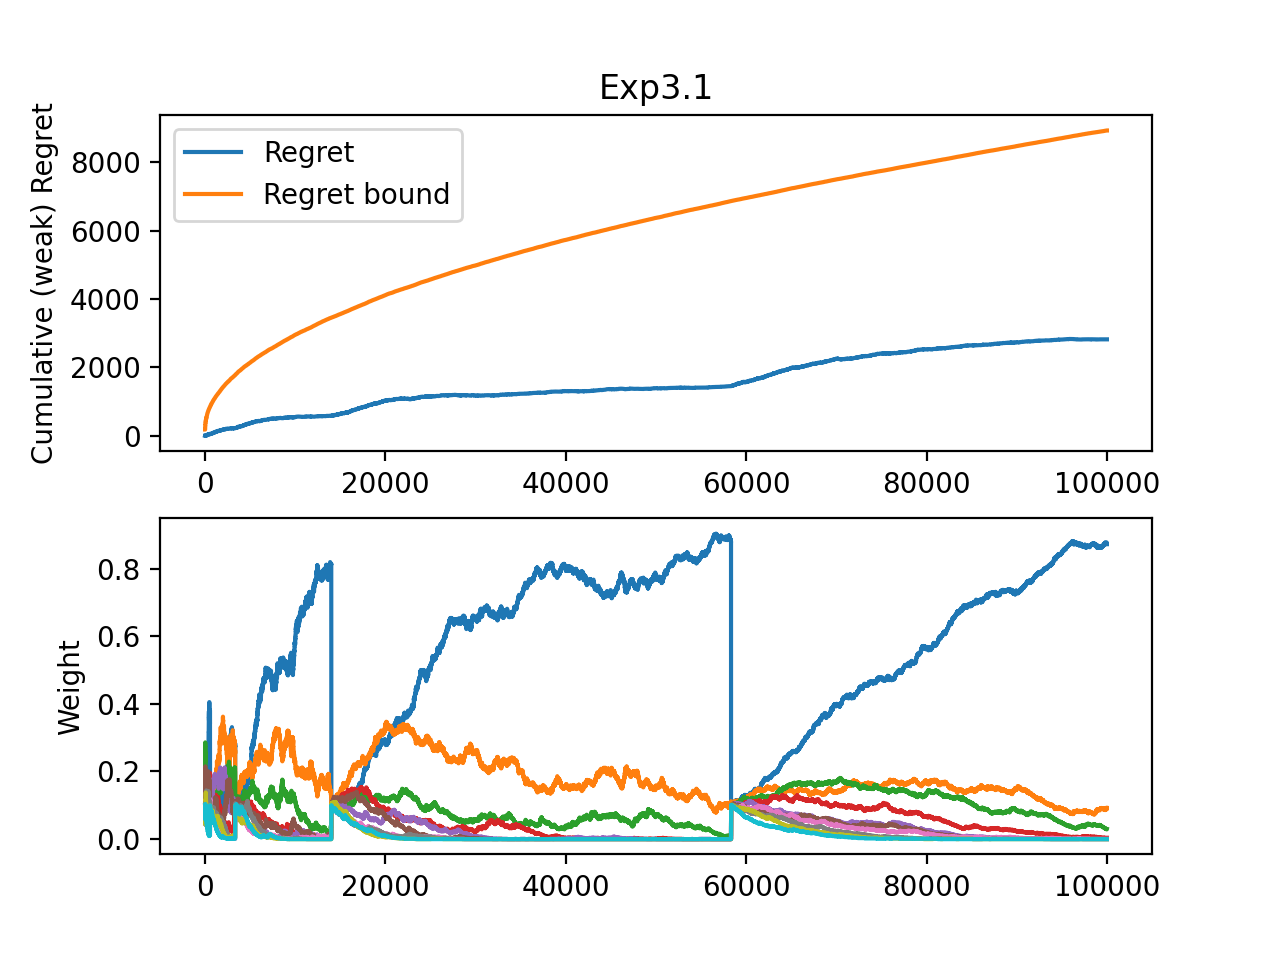
\includegraphics[width=90mm, height=70mm]{exp31.png}
		\caption{We can observe the weights being reset at each epoch. Also, it appears to converge faster to the optimal arm (weight in blue) for each successive epoch}
	\end{center}
\end{figure}
Each epoch is clearly visible, since the weights are reset to 1. As expected, \textbf{Exp3.1} has a higher regret than \textbf{Exp3}. This is caused by the loss of information about $T$.

We also show the performance of \textbf{Exp3.P} on the same dataset (Figure 3). As we can see, the theoretical bound on the regret is significantly higher compared to \textbf{Exp3}. However, in this particular instance, we are well below the theoretical bound, performing only slightly worse than \textbf{Exp3}.
\begin{figure}[!htb]
	\begin{center}
		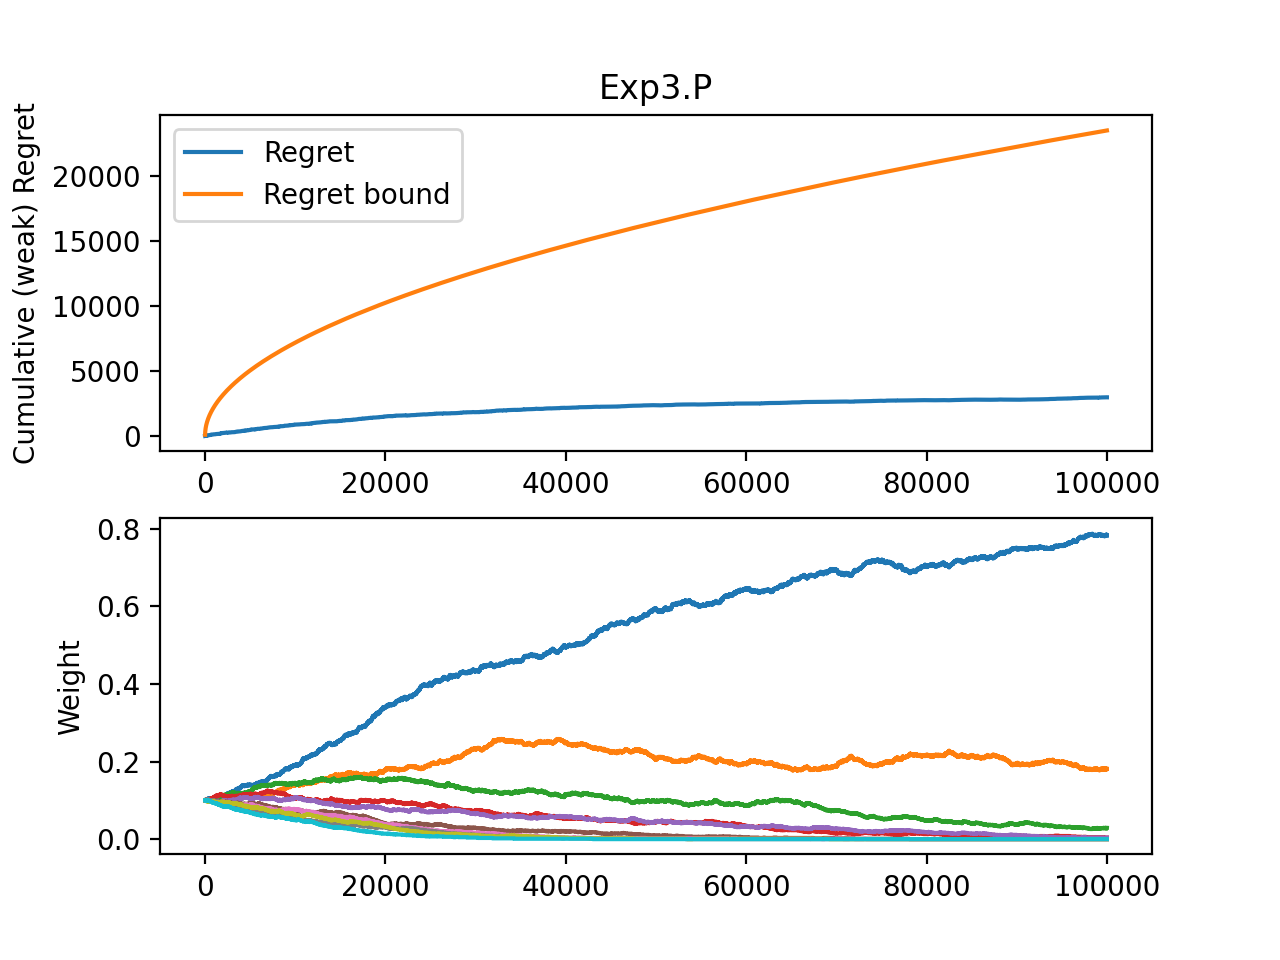
\includegraphics[width=90mm, height=70mm]{exp3P.png}
		\caption{The theoretical upper bound is much higher than those of \textbf{Exp3} and \textbf{Exp3.1}. However, the actual regret in this realization is approximately 2500}
	\end{center}
\end{figure}

These results are of course subject to the randomness of the algorithms, and performance may vary significantly from realization to realization.

\section{Advantages and Drawbacks}

The paper starts by presenting the adversarial setting and the necessity of dropping the stochasticity assumption.  It proposes an efficient algorithm to solve the problem. However, it also adapts it to work in environments where some variables are unknown, such as the time horizon $T$ (solved with \textbf{Exp3.1}).

Additionally, the paper addresses less obvious issues that can impact performance, such as the variance of the expected regret. To mitigate this problem, the authors propose \textbf{Exp3.P}.  A strong point of this work is the wide selection of \textbf{Exp3} variants shown, especially considering the scarcity of literature on the subject at the time of publication.

The paper adequately presents the non-trivial mathematical instruments required for each proof, e.g., well-known inequalities. An example is the use of Jensen's inequality in the proof of the bound for \textbf{Exp3.1}, that is, given a random variable $X$ and a convex function $\varphi$, then $\varphi(\mathbb{E}[X]) \leq \mathbb{E}[\varphi(X)]$.


Clarity of execution is greatly appreciated, with careful justification of every non-obvious step, given the depth and rigor required for each proof.

The final part on applications to game theory is adequately motivated and coherent with the previous results.

The main weakness of this work is perhaps the abrupt switch to \textbf{Exp4} and \textbf{Exp3.S}. Both variants are not as natural as \textbf{Exp3.1}, \textbf{Exp3.P}, and \textbf{Exp3.P.1}. They seem to be preliminary work for a more complete analysis, and they lack additional context. For example, there is no variant of \textbf{Exp4} that guarantees a regret bound with high probability. Beygelzimer \cite{pmlr-v15-beygelzimer11a}, using a similar technique to \textbf{Exp3.P}, proposed \textbf{Exp4.P}, which addresses this issue. 

\section{Improvements and Extensions}

Over 20 years have passed since the publication of this work, a wide family of algorithms has been developed, and the setting has been further extended.

An open question is whether the degree of exploration can be reduced without compromising performance. For example, in a problem with many suboptimal arms, a significant amount of time may be wasted despite continuously adapting drawing distributions. Recently, Neu \cite{neu} proposed "implicit exploration" techniques, which aim to minimize the number of necessary draws for an optimal guarantee.

We can also consider a hybrid setting where we have stochastic and adversarial rewards at intervals, which is also referred to as "adversarial corruption." The problem has been studied in Altschuler \cite{alts}, Kapoor \cite{kapoor}, and Jun\cite{jun}. An interesting solution that achieves (almost) optimal regret in both cases is the \textbf{SOA} algorithm (Bubeck et al. \cite{seb}). However, it does not directly address the corruption problem. Gupta \cite{guptakoren} recently proposed \textbf{BARBAR}, an algorithm capable of handling adversarial corruption up to a constant $C$. It achieves regret (with high probability) of $O(KC + \sum_{i\neq i^\star}^{}\frac{\log T}{\Delta_i}\log(\frac{K}{\delta}\log T))$.

The setting can be further enriched by allowing the adversary to adapt to our actions. Formally, this means that the adversarial choice of assigning a reward at round $t$ is a function of our previous actions (i.e., the arms pulled at rounds $t-1, t-2, \dots$). Dekel et al. \cite{dekel} proposed a new notion of regret for addressing this problem called policy regret.

Lastly, we can also encounter situations where we have information about the other arms' rewards. This is a common occurence in web advertising or sensor networks for example.  Graph-based approaches for modelling the relationship between the rewards have been developed by Mannor \cite{mannor} and Alon et al. \cite{alon}.


\bibliographystyle{plain}
\bibliography{references} 

\end{document}